% !TEX program = xelatex
% 中英对照译文：An EEG dataset for studying asynchronous SSVEP-based brain computer interfaces
% 用途：个人学习（原文为 CC BY 4.0 开放获取论文）
\documentclass[11pt]{ctexart}
\usepackage[a4paper,margin=2.2cm]{geometry}
\usepackage{amsmath,amssymb}
\usepackage{booktabs}
\usepackage{graphicx}
\usepackage{xcolor}
\usepackage{enumitem}
\usepackage[most]{tcolorbox}
\usepackage[colorlinks=true,linkcolor=blue!55!black,urlcolor=blue!55!black,citecolor=blue!55!black]{hyperref}

\setlist{nosep,leftmargin=2em}
\setlength{\parskip}{2pt}

% ---------- 英文原文框 ----------
\newtcolorbox{enbox}{
  enhanced, breakable,
  colback=gray!3, colframe=gray!55,
  boxrule=0pt, leftrule=2.5pt, arc=1pt,
  left=7pt, right=6pt, top=3pt, bottom=3pt,
  before skip=6pt, after skip=2pt
}
% ---------- 中文译文框 ----------
\newtcolorbox{zhbox}{
  enhanced, breakable,
  colback=blue!4, colframe=blue!45!black,
  boxrule=0pt, leftrule=2.5pt, arc=1pt,
  left=7pt, right=6pt, top=3pt, bottom=3pt,
  before skip=2pt, after skip=10pt
}
\newenvironment{en}{\begin{enbox}\color{black!85}}{\end{enbox}}
\newenvironment{zh}{\begin{zhbox}}{\end{zhbox}}

% 译注
\newcommand{\tnote}[1]{\textcolor{gray}{\small（译注：#1）}}

\title{}
\author{}
\date{}

\begin{document}

% ================= 标题区 =================
\begin{center}
{\LARGE\bfseries An EEG dataset for studying asynchronous steady-state visual evoked potential (SSVEP) based brain computer interfaces\par}
\vspace{6pt}
{\Large\bfseries 用于研究基于异步稳态视觉诱发电位（SSVEP）脑机接口的脑电（EEG）数据集\par}
\vspace{10pt}
{\normalsize Jing Zhao$^{a}$, Qian Zhang$^{a}$, Xinrui Wang$^{b}$, Xueshuo Liu$^{a}$, Jiaxin Li$^{a}$, Fengjie Fan$^{a}$, Zhenhu Liang$^{a}$, Xiaoli Li$^{c,d}$\par}
\vspace{4pt}
{\small
$^{a}$~燕山大学电气工程学院（Department of Electrical Engineering, Yanshan University），中国秦皇岛\\
$^{b}$~清华大学苏州汽车研究院（Suzhou Automobile Research Institute, Tsinghua University），中国苏州\\
$^{c}$~广东省人工智能与数字经济实验室（广州）（Guangdong Artificial Intelligence and Digital Economy Laboratory, Guangzhou），中国广州\\
$^{d}$~华南理工大学自动化科学与工程学院（School of Automation Science and Engineering, South China University of Technology），中国广州\par}
\vspace{8pt}
{\small \textit{Brain-Apparatus Communication: A Journal of Bacomics}, 2024, 3(1): 2418650\\
DOI: \href{https://doi.org/10.1080/27706710.2024.2418650}{10.1080/27706710.2024.2418650} \quad 在线发表：2024 年 10 月 26 日\par}
\end{center}

\vspace{2pt}
\noindent\textcolor{gray}{\rule{\textwidth}{0.4pt}}
\vspace{2pt}

\noindent{\small\textbf{文章历史（Article History）}\quad 收稿日期：2024 年 1 月 2 日；录用日期：2024 年 10 月 6 日\\
\textbf{联系作者（CONTACT）}\quad Xiaoli Li, xiaolili@scut.edu.cn，华南理工大学自动化科学与工程学院，广州 510641\\
\textbf{版权说明}\quad © 2024 The Author(s)。本文为开放获取文章，依据知识共享署名许可协议（Creative Commons Attribution License, \href{https://creativecommons.org/licenses/by/4.0/}{CC BY 4.0}）发布，允许在任何媒介中不受限制地使用、分发与复制，前提是正确引用原始作品。}

\vspace{4pt}
\begin{enbox}\small\color{gray}
译者说明：本文档为个人初学者研究学习用途的中英对照译文，原文为上述开放获取（CC BY 4.0）论文。译文仅供理解参考，如有歧义请以英文原文为准。专业术语首次出现时保留英文缩写；参考文献保留原文以便检索核对。
\end{enbox}

% ================= 摘要 =================
\section*{摘要（ABSTRACT）}
\begin{en}
Compared with the commonly used synchronous brain-computer interface (BCI), the asynchronous BCI is a more flexible and natural way to control the real-world robotic devices. The major difficulty of building a robust asynchronous BCI lies in the discrimination between control states (CSs) and non-control states (NSs). This article presents an open-source 63-channel electroencephalogram (EEG) dataset of 24 subjects for asynchronous steady-state visual evoked potential (SSVEP)-BCI research. The data was recorded from an SSVEP based CS task and three different types of NS tasks, namely NS1, NS2 and NS3. The dataset was evaluated using three processes, including analysis of temporal waveform, amplitude spectrum and signal-to-noise (SNR), recognition of SSVEP frequencies, and classification between CS and NS. The dataset can be used to support studies of asynchronous classification, NS detection, and discrimination between different NSs.
\end{en}
\begin{zh}
与常用的同步脑机接口（brain-computer interface, BCI）相比，异步 BCI 是一种更为灵活、自然的现实世界机器人设备控制方式。构建鲁棒的异步 BCI 的主要难点在于区分控制状态（control state, CS）与非控制状态（non-control state, NS）。本文发布了一个开源的 63 通道脑电图（electroencephalogram, EEG）数据集，包含 24 名被试，用于异步稳态视觉诱发电位（steady-state visual evoked potential, SSVEP）BCI 研究。数据采集自一项基于 SSVEP 的 CS 任务和三种不同类型的 NS 任务，即 NS1、NS2 与 NS3。该数据集通过三个流程进行评估：时域波形、幅值谱与信噪比（signal-to-noise ratio, SNR）分析，SSVEP 频率识别，以及 CS 与 NS 之间的分类。该数据集可用于支持异步分类、NS 检测以及不同 NS 之间区分的研究。
\end{zh}

\noindent\textbf{关键词：}脑机接口（BCI）；脑电图（EEG）；稳态视觉诱发电位（SSVEP）；异步；非控制状态（NS）

% ================= 1 引言 =================
\section{引言（Introduction）}

\begin{en}
Brain-computer interface (BCI) provides a direct communication pathway between human brain and computer devices. In the current electroencephalogram (EEG)-based BCIs, steady-state visual evoked potential (SSVEP) is a paradigm widely used for control of robots because of its high information transfer rate (ITR) and low training demands [1, 2]. Several visual stimuli, corresponding to different commands to control a robot, are flickering at different frequencies on a user interface to evoke the SSVEP responses [2--5].
\end{en}
\begin{zh}
脑机接口（BCI）在人脑与计算机设备之间提供了一条直接的通信通路。在现有基于脑电图（EEG）的 BCI 中，稳态视觉诱发电位（SSVEP）因其信息传输速率（information transfer rate, ITR）高、训练需求低，被广泛用作控制机器人的范式 [1, 2]。在用户界面上，若干对应不同机器人控制指令的视觉刺激以不同频率闪烁，从而诱发 SSVEP 响应 [2--5]。
\end{zh}

\begin{en}
To classify the SSVEP signals, both synchronous methods and asynchronous methods are developed. The synchronous methods [6--10] are designed to identify only the frequency or phase components related to the flickering stimuli, while the asynchronous methods [11--15] also recognize the control state (CS) and non-control state (NS) in the SSVEP task. Compared with the synchronous method, the asynchronous method enables the participant to start and stop the control task (for SSVEP, fixating on the stimulus) at will, and is a more flexible and natural way to control the real-world robotic devices. But in an asynchronous BCI, as the participant is allowed to perform any mental activity other than fixating on stimuli during the non-control period, the major difficulty lies in the discrimination between the CSs and NSs [16].
\end{en}
\begin{zh}
为对 SSVEP 信号进行分类，研究者已发展出同步方法与异步方法。同步方法 [6--10] 旨在仅识别与闪烁刺激相关的频率或相位成分，而异步方法 [11--15] 还能识别 SSVEP 任务中的控制状态（CS）与非控制状态（NS）。与同步方法相比，异步方法允许被试随意启动和停止控制任务（对 SSVEP 而言即注视刺激），是一种更为灵活、自然的现实世界机器人设备控制方式。但在异步 BCI 中，由于被试在非控制期间可以执行除注视刺激之外的任何心理活动，主要难点在于区分 CS 与 NS [16]。
\end{zh}

\begin{en}
Although there are several datasets [17--20] published for SSVEP-related research, NS trials in these datasets are usually recorded with small amount and short duration. Therefore, these datasets are more suitable for synchronous SSVEP research than for asynchronous research which requires a certain amount of NS data. The motivation of this article is to publish an open-source dataset with a large quantity and variety of NS data, and validate its effectiveness in offline classification study, to facilitate asynchronous SSVEP research. This study presents an open-source 63-channel EEG dataset of 24 subjects for asynchronous SSVEP-BCI research. The data was recorded from an SSVEP based CS task and three different types of NS tasks, namely NS1, NS2 and NS3. In the CS task, the subjects were asked to stare at a target stimulus for evoking SSVEP responses. In the three NS tasks, the subjects were asked to focus on the feedback image of a camera when the stimuli are not flickering, watch the white wall for a rest, and watch the feedback image when the stimuli are flickering continuously, respectively. For each subject, all the data was recorded within three hours and a short break was allowed between two neighboring sessions. Event markers were accurately synchronized to the recording of EEG data. This dataset contained the data epochs extracted from the recorded raw data without pre-processing. The data could be further pre-processed according to the researchers' needs. The dataset supports in-depth study of artifact denoising, SSVEP recognition, NS detection, and discrimination between different NSs.
\end{en}
\begin{zh}
尽管已有若干面向 SSVEP 相关研究的数据集 [17--20] 发布，但这些数据集中的 NS 试次通常数量少、时长短。因此，这些数据集更适合同步 SSVEP 研究，而不太适合需要一定数量 NS 数据的异步研究。本文的动机在于发布一个包含大量且多样化 NS 数据的开源数据集，并通过离线分类研究验证其有效性，以促进异步 SSVEP 研究。本研究发布了一个包含 24 名被试的开源 63 通道 EEG 数据集，用于异步 SSVEP-BCI 研究。数据采集自一项基于 SSVEP 的 CS 任务和三种不同类型的 NS 任务，即 NS1、NS2 与 NS3。在 CS 任务中，要求被试注视目标刺激以诱发 SSVEP 响应。在三种 NS 任务中，分别要求被试在刺激不闪烁时注视摄像头的反馈图像、观看白墙休息，以及在刺激持续闪烁时观看反馈图像。每位被试的全部数据在三小时内采集完成，相邻两个区组（session）之间允许短暂休息。事件标记（event marker）与 EEG 数据记录精确同步。该数据集包含从记录的原始数据中提取、未经预处理的数据片段（epoch），研究者可根据自身需要进一步预处理。该数据集支持对伪迹去噪、SSVEP 识别、NS 检测以及不同 NS 之间区分的深入研究。
\end{zh}

\begin{en}
In this study, we validated the dataset using three evaluation processes, i.e., analysis of temporal waveform, amplitude spectrum and signal-to-noise (SNR), recognition of SSVEP frequencies, and classification between CS and NS. To evaluate the recognition performance of SSVEP frequencies, this study used three algorithms commonly used in SSVEP research, including filter-bank canonical correlation analysis (FBCCA) [8], task-related component analysis (TRCA) [7], and ensembled task-related component analysis (eTRCA) [7]. To evaluate the classification performance between the CS and NS, this study used two commonly used algorithms, i.e., individualized frequency band based optimized complex network (IFB-OCN) [12] and frequency specific framework using ensembled task-related component analysis (FS-eTRCA) [13]. An extension of the FS-eTRCA algorithm namely FS-eTRCA\&FBCCA was also used for evaluation of discrimination performance between the CS and NS.
\end{en}
\begin{zh}
本研究通过三个评估流程对数据集进行验证，即时域波形、幅值谱与信噪比（SNR）分析，SSVEP 频率识别，以及 CS 与 NS 之间的分类。为评估 SSVEP 频率的识别性能，本研究采用了 SSVEP 研究中常用的三种算法：滤波器组典型相关分析（filter-bank canonical correlation analysis, FBCCA）[8]、任务相关成分分析（task-related component analysis, TRCA）[7] 与集成任务相关成分分析（ensembled task-related component analysis, eTRCA）[7]。为评估 CS 与 NS 之间的分类性能，本研究采用了两种常用算法，即基于个体化频带的优化复杂网络（individualized frequency band based optimized complex network, IFB-OCN）[12] 和采用 eTRCA 的频率特定框架（frequency specific framework using ensembled task-related component analysis, FS-eTRCA）[13]。此外，还使用了 FS-eTRCA 算法的一种扩展形式 FS-eTRCA\&FBCCA 来评估 CS 与 NS 的区分性能。
\end{zh}

\begin{en}
The remainder of this article is outlined as follows. The Methods Section introduces the subjects, stimulus presentation, experimental paradigm, and acquisition settings to record the dataset. The Data Records Section describes the related information of the dataset helpful for sharing. The Performance Evaluation Section presents the temporal, frequency and spatial features of the dataset and validates its effectiveness for asynchronous SSVEP classification. The Discussion Section discusses some issues that arose from this study and other notes, and gives suggestions for future work. The Conclusion Section summarizes the article. The dataset can be downloaded via the link provided by figshare [21].
\end{en}
\begin{zh}
本文其余部分安排如下：方法（Methods）部分介绍记录该数据集所涉及的被试、刺激呈现、实验范式与采集设置；数据记录（Data Records）部分介绍有助于数据共享的数据集相关信息；性能评估（Performance Evaluation）部分给出数据集的时域、频域与空间域特征，并验证其在异步 SSVEP 分类中的有效性；讨论（Discussion）部分讨论本研究中出现的一些问题及其他注意事项，并对未来工作提出建议；结论（Conclusion）部分对全文进行总结。数据集可通过 figshare 提供的链接下载 [21]。
\end{zh}

% ================= 2 方法 =================
\section{方法（Methods）}

\subsection{被试（Subjects）}
\begin{en}
Twenty-four healthy individuals (9 females, aged 18--27 years, mean age: 22.96 years) took part in the experiment. All subjects had normal or corrected-to-normal vision and had no cognitive or psychological issues. Before the experiment, all subjects thoroughly understood the experimental procedures and signed written informed consent. The subjects were paid after the experiment. This study was reviewed and approved by the ethics committee of Qinhuangdao First Hospital.
\end{en}
\begin{zh}
24 名健康个体（女性 9 名，年龄 18--27 岁，平均年龄 22.96 岁）参加了实验。所有被试视力正常或矫正至正常，无认知或心理问题。实验前，所有被试均已充分了解实验流程并签署书面知情同意书。被试在实验结束后获得报酬。本研究经秦皇岛市第一医院伦理委员会审查批准。
\end{zh}

\subsection{刺激呈现（Stimulus Presentation）}
\begin{en}
The experiment involved presenting visual stimuli on a 23.6-inch LCD monitor with a resolution of $1920\times1080$ pixels at 60 Hz. The stimulation program was developed in MATLAB (MathWorks, Inc.) using the Psychophysics Toolbox Version 3 (PTB-3) [22]. Eight stimuli were modulated by sinusoidal modulation signals at frequencies of 8 Hz, 9 Hz, 10.5 Hz, 11 Hz, 12 Hz, 13 Hz, 14 Hz and 15 Hz, respectively. Figure 1 shows the stimulation interface involved the SSVEP task. The eight flickering stimuli were arranged in a $3\times3$ matrix, and a feedback image was displayed at the center of the interface.
\end{en}
\begin{zh}
实验在一台 23.6 英寸液晶显示器上呈现视觉刺激，分辨率为 $1920\times1080$ 像素，刷新率 60 Hz。刺激程序基于 MATLAB（MathWorks 公司）并使用心理物理学工具箱第 3 版（Psychophysics Toolbox Version 3, PTB-3）[22] 开发。八个刺激分别由频率为 8 Hz、9 Hz、10.5 Hz、11 Hz、12 Hz、13 Hz、14 Hz 和 15 Hz 的正弦调制信号进行调制。图 1 展示了 SSVEP 任务所用的刺激界面。八个闪烁刺激按 $3\times3$ 矩阵排列，界面中央显示反馈图像。
\end{zh}

\begin{en}
The control signal for each stimulus was generated by a sampled sinusoidal stimulation method [23]. At frequency $f$ and phase $\theta$, the stimulus sequence $s(f,\theta,i)$ can be generated by modulating the luminance of the screen.
\end{en}
\begin{zh}
每个刺激的控制信号由采样正弦刺激方法 [23] 生成。在频率 $f$ 和相位 $\theta$ 下，可通过调制屏幕亮度生成刺激序列 $s(f,\theta,i)$：
\end{zh}

\begin{equation}
s(f,\theta,i)=\frac{1}{2}\left[1+\sin\left(2\pi f\,\frac{i}{\mathrm{RefreshRate}}+\theta\right)\right]
\end{equation}

\begin{en}
where $\sin(\cdot)$ generates a sine wave, $i$ indicates the frame index in the sequence, and the refresh rate of the LCD monitor was 60 Hz. In the stimulus sequence, 0 denotes darkness and 1 denotes peak luminance. In this study, the phase $\theta$ was set to 0 for all the stimulation frequencies.
\end{en}
\begin{zh}
其中 $\sin(\cdot)$ 生成正弦波，$i$ 表示序列中的帧索引，液晶显示器刷新率为 60 Hz。在刺激序列中，0 表示全暗，1 表示峰值亮度。本研究中，所有刺激频率的相位 $\theta$ 均设为 0。
\end{zh}

\begin{center}
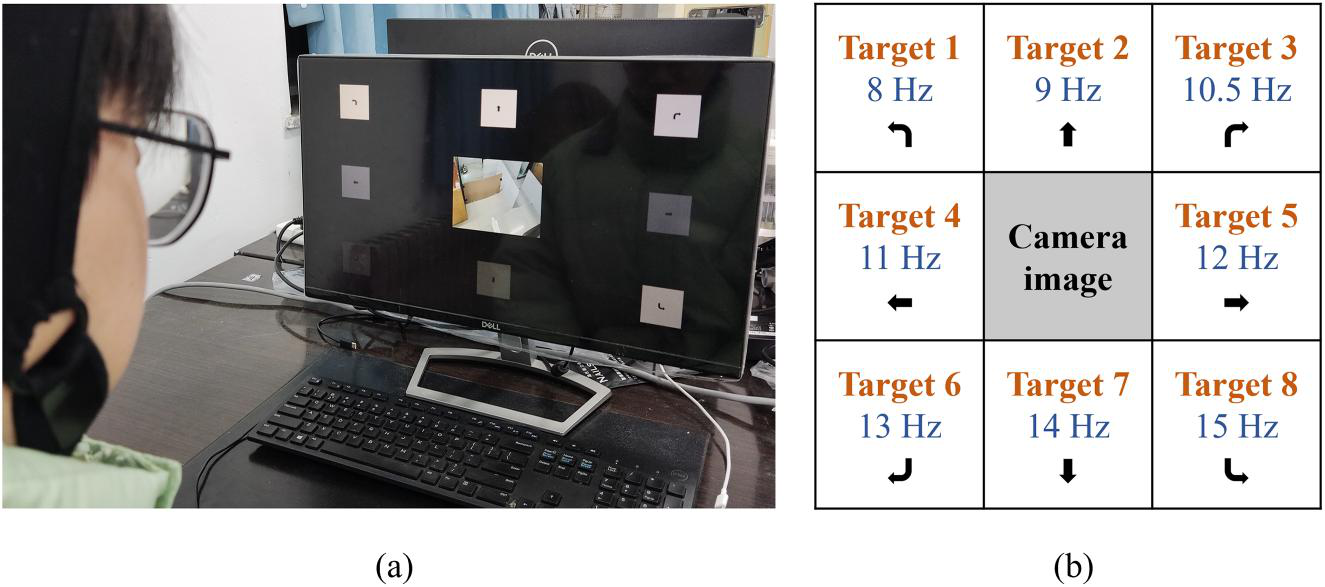
\includegraphics[width=0.92\textwidth]{figs/fig1.png}
\end{center}
\begin{en}
\textbf{Figure 1.} Stimulation interface. (a) Interface involved SSVEP stimulation. (b) Frequency values (phase value $= 0$) and location of stimuli.
\end{en}
\begin{zh}
\textbf{图 1.} 刺激界面。(a) 包含 SSVEP 刺激的界面；(b) 刺激的频率值（相位值 $=0$）与位置。
\end{zh}

\subsection{实验范式（Experimental Paradigm）}
\begin{en}
Before the experiment, each subject was explained the experimental procedures and had a thorough understanding of the whole process. Meanwhile, the experimenter ensured reliability by monitoring the whole experimental process. The experiment was carried out in a laboratory environment without electromagnetic shielding. The subjects sat on an armchair 0.5 m away from the LCD monitor, and conducted an offline experiment to acquire the EEG data of the four states. In the experiment, the subject was instructed to perform the corresponding tasks, respectively. Figure 2 shows the experimental procedure of performing the four tasks. Between tasks, there was a break lasting several seconds or several minutes depending on subjects' preference.
\end{en}
\begin{zh}
实验前，向每位被试讲解实验流程，使其对整个过程有充分了解。同时，实验员通过全程监督来保证实验的可靠性。实验在无电磁屏蔽的实验室环境中进行。被试坐在距液晶显示器 0.5 m 的扶手椅上，进行离线实验以采集四种状态的 EEG 数据。实验中，被试被要求分别执行相应任务。图 2 展示了执行四项任务的实验流程。任务之间有持续数秒至数分钟的休息，时长取决于被试的个人意愿。
\end{zh}

\begin{enumerate}[label=\textbf{\arabic*.}]
\item \textbf{CS 任务（CS task）}
\begin{en}
In the CS task, the subjects conducted a total of three sessions of the SSVEP experiment. Each session contained three blocks, each consisting of eight trials. Between sessions, the subjects were allowed to take a break lasting seconds or minutes as they wished. At the beginning of each trial, the user interface selected one stimulus as the target, following the order from lower frequency to higher frequency, and highlighted it with a static green square. After 1.5 s, the green square disappeared and the interface started to flicker the 8 stimuli for 4 s. During this 4-s period, the subjects were asked to stare at the target stimulus while avoiding possible body movements and eyeblinks. After that, the interface stopped the flickering of the stimuli, and the subjects took a rest for 0.5 s. The 4.5-s data epochs after the start of flickering were extracted for this dataset, consisting of a 4-s CS task and a 0.5-s break.
\end{en}
\begin{zh}
在 CS 任务中，被试共进行三个区组（session）的 SSVEP 实验。每个区组包含三个 block，每个 block 包含八个试次（trial）。区组之间允许被试按自己的意愿休息数秒或数分钟。每个试次开始时，用户界面按从低频到高频的顺序选择一个刺激作为目标，并用静态绿色方框将其高亮。1.5 s 后绿色方框消失，界面开始以 4 s 时长闪烁 8 个刺激。在这 4 s 内，要求被试注视目标刺激，同时尽量避免身体运动和眨眼。此后界面停止刺激闪烁，被试休息 0.5 s。本数据集提取闪烁开始后的 4.5 s 数据片段，包含 4 s 的 CS 任务和 0.5 s 的休息。
\end{zh}

\item \textbf{NS1 任务（NS1 task）}
\begin{en}
The NS1 task was conducted using a similar stimulation program to the CS task, but the eight stimuli were not flickering during the whole task. The subjects were asked to watch the image feedback in the middle of the interface when the task started, taking no break during the NS1 task. Each subject conducted three blocks of NS1 tasks, each consisting of eight trials. The 4-s data epoch from 1.5 s to 5.5 s (0 indicates the start of a trial) of each trial were extracted as the NS1 task for this dataset.
\end{en}
\begin{zh}
NS1 任务采用与 CS 任务类似的刺激程序，但八个刺激在整个任务期间不闪烁。任务开始时，要求被试观看界面中央的反馈图像，且在 NS1 任务期间不休息。每位被试进行三个 block 的 NS1 任务，每个 block 包含八个试次。本数据集提取每个试次 1.5 s 至 5.5 s（0 表示试次开始）的 4 s 数据片段作为 NS1 任务数据。
\end{zh}

\item \textbf{NS2 任务（NS2 task）}
\begin{en}
The NS2 task was conducted using the same stimulation program as the CS task. Different from the CS task, the NS2 task asked the subjects to watch the white wall and take a rest during the NS2 task. The 4-s data epochs from 1.5 s to 5.5 s (0 indicates the start of a trial) of each trial were extracted as the NS2 task for this dataset.
\end{en}
\begin{zh}
NS2 任务采用与 CS 任务相同的刺激程序。与 CS 任务不同的是，NS2 任务要求被试在任务期间观看白墙并休息。本数据集提取每个试次 1.5 s 至 5.5 s（0 表示试次开始）的 4 s 数据片段作为 NS2 任务数据。
\end{zh}

\item \textbf{NS3 任务（NS3 task）}
\begin{en}
The NS3 task was carried out using an asynchronous SSVEP paradigm. As shown in Figure 2, all the stimuli were flickering continuously for the whole task. The NS3 task required the subjects to watch the image feedback of surroundings for decisions making of subsequent commands. To acquire EEG data of the NS3 task, the subjects had to focus on the feedback image in the middle of the interface for 2 s. The interface then displayed a green square for 3 s to instruct the subjects to stare at the corresponding stimulus target. After that, the green indicator disappeared to start the next trial, and the subjects had to switch their gaze to the feedback image. Each subject conducted two sessions of the NS3 tasks, consisting of a total of 48 trials. The 2-s data epochs of focusing on the feedback image were extracted as the NS3 task for this dataset.
\end{en}
\begin{zh}
NS3 任务采用异步 SSVEP 范式。如图 2 所示，所有刺激在整个任务期间持续闪烁。NS3 任务要求被试观看周围环境的反馈图像，以便对后续指令作出决策。为采集 NS3 任务的 EEG 数据，被试需注视界面中央的反馈图像 2 s；随后界面显示绿色方框 3 s，指示被试注视相应的刺激目标；此后绿色指示消失并开始下一试次，被试需将视线转回反馈图像。每位被试进行两个区组的 NS3 任务，共 48 个试次。本数据集提取注视反馈图像的 2 s 数据片段作为 NS3 任务数据。
\end{zh}
\end{enumerate}

\begin{center}
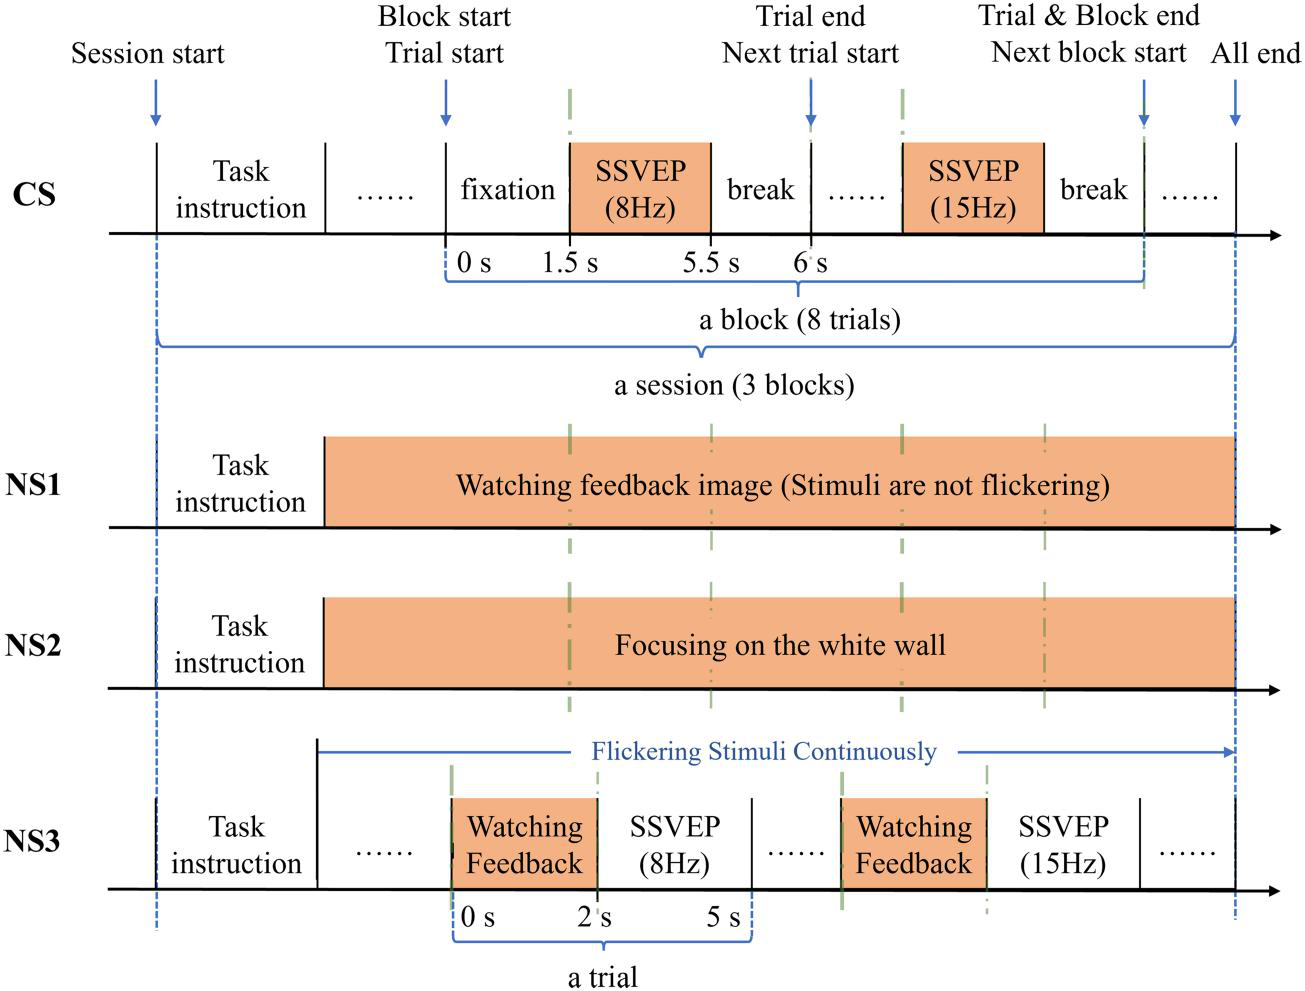
\includegraphics[width=0.95\textwidth]{figs/fig2.png}
\end{center}
\begin{en}
\textbf{Figure 2.} Experimental procedure of recording EEG data under different states. The orange color indicates the state we aim to record. The pairs of green-colored dashed lines indicate the data we extracted: the bolder line indicated the start of an extraction, and the finer line indicated the end of an extraction. For the NS1 and NS2 tasks, the data epochs were extracted using the same time as SSVEP focusing period in the CS task.
\end{en}
\begin{zh}
\textbf{图 2.} 不同状态下 EEG 数据记录的实验流程。橙色表示我们想要记录的状态。成对的绿色虚线表示我们提取的数据：较粗的线表示提取起点，较细的线表示提取终点。NS1 与 NS2 任务的数据片段提取时间与 CS 任务中 SSVEP 注视期的时间一致。
\end{zh}

\subsection{数据采集与预处理（Data Acquisition and Preprocessing）}
\begin{en}
This study used a 63 channel actiCHamp EEG system (Brain products, Germany) to record EEG data at a sampling rate of 5000 Hz. Electrodes were placed according to the international 10--20 system. The reference electrode was placed at Fz and the ground electrode was placed at FPz. Electrode impedances were kept below 50~k$\Omega$ during recording. The electrode placement of the EEG cap was shown in Figure 3.
\end{en}
\begin{zh}
本研究使用 63 通道 actiCHamp EEG 系统（Brain Products，德国）以 5000 Hz 采样率记录 EEG 数据。电极按国际 10--20 系统（international 10--20 system）放置，参考电极置于 Fz，接地电极置于 FPz。记录过程中电极阻抗保持在 50~k$\Omega$ 以下。EEG 电极帽的电极位置如图 3 所示。
\end{zh}

\begin{en}
Data epochs of the four tasks were extracted from the recorded raw data. For the CS task, each epoch contained a 4.5-s EEG data corresponding to the 4-s SSVEP focusing and 0.5-s break; For the NS1 task, each epoch contained a 4-s EEG data recorded during watching the feedback image when the stimuli were not flickering; For the NS2 task, each epoch contained a 4-s EEG data recorded during gazing at the white wall. For the NS3 task, each epoch contained a 2-s EEG data recorded during gazing at the feedback image in the asynchronous SSVEP paradigm. Table 1 lists the detailed information of the dataset.
\end{en}
\begin{zh}
从记录的原始数据中提取四项任务的数据片段。CS 任务中，每个片段包含 4.5 s 的 EEG 数据，对应 4 s 的 SSVEP 注视和 0.5 s 的休息；NS1 任务中，每个片段包含刺激不闪烁时观看反馈图像期间记录的 4 s EEG 数据；NS2 任务中，每个片段包含注视白墙期间记录的 4 s EEG 数据；NS3 任务中，每个片段包含异步 SSVEP 范式下注视反馈图像期间记录的 2 s EEG 数据。表 1 列出了数据集的详细信息。
\end{zh}

\begin{table}[htbp]
\centering
\caption{数据集详细信息（Table 1. Detailed information of the dataset）}
\begin{tabular}{ll}
\toprule
参数（Parameters） & 数值（Values） \\
\midrule
被试数量（Number of subjects） & 24 \\
采样率（Sampling rate） & 5000 Hz \\
通道数（Number of channels） & 63 \\
类别数（Number of classes） & 4（CS, NS1, NS2, NS3） \\
\bottomrule
\end{tabular}
\end{table}

\begin{center}
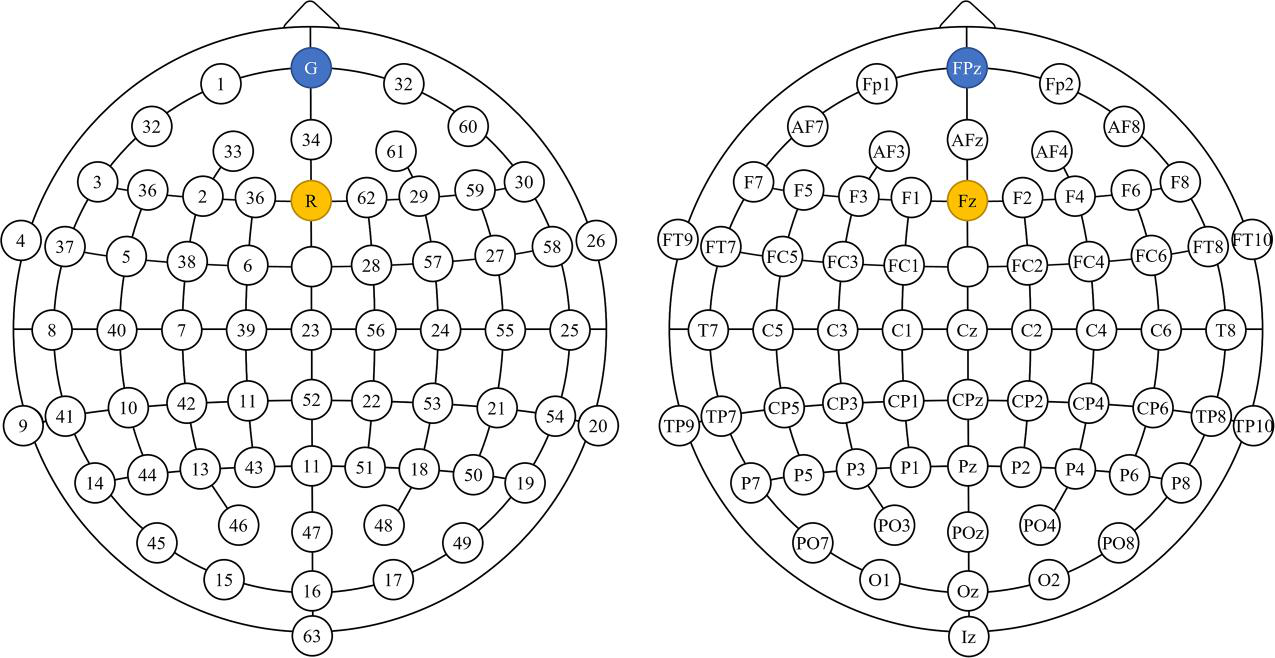
\includegraphics[width=0.85\textwidth]{figs/fig3.png}
\end{center}
\begin{en}
\textbf{Figure 3.} Electrode placement of the dataset.
\end{en}
\begin{zh}
\textbf{图 3.} 数据集的电极位置。
\end{zh}

% ================= 3 数据记录 =================
\section{数据记录（Data Records）}

\subsection{EEG 数据（EEG Data）}
\begin{en}
Data were stored as double precision floating-point values in MATLAB. There are 24 folders named ``Sxx'' for each subject (i.e., S01, S02, \ldots, S24). For each ``Sxx'' folder, the EEG data for the corresponding subject of the four tasks was saved as a ``.mat'' file respectively. The file naming rules were as follows:
\end{en}
\begin{zh}
数据以双精度浮点数值存储于 MATLAB 文件中。共有 24 个以 ``Sxx'' 命名的文件夹，对应各被试（即 S01、S02、\ldots、S24）。每个 ``Sxx'' 文件夹中，该被试四项任务的 EEG 数据分别保存为一个 ``.mat'' 文件。文件命名规则如下：
\end{zh}

\begin{center}
\texttt{sub\_xx\_data\_yyy.mat}
\end{center}

\begin{en}
where ``xx'' was the subject number (01, 02, \ldots, 24), ``yyy'' represented the control and non-control tasks including CS, NS1, NS2, and NS3. The following data matrices were loaded in MATLAB by loading the corresponding ``.mat'' files.
\end{en}
\begin{zh}
其中 ``xx'' 为被试编号（01、02、\ldots、24），``yyy'' 表示控制与非控制任务，包括 CS、NS1、NS2 和 NS3。在 MATLAB 中加载相应的 ``.mat'' 文件即可读取以下数据矩阵。
\end{zh}

\begin{itemize}
\item \texttt{data\_CS}
\begin{en}
consisting of 96 trials of EEG data recorded in the CS task. The data size was $8\times63\times22500\times12$ (target numbers, channel numbers, data samples and trial numbers). The eight targets correspond to the stimulation frequencies of 8 Hz, 9 Hz, 10.5 Hz, 11 Hz, 12 Hz, 13 Hz, 14 Hz and 15 Hz, respectively. The 22500 samples consisted of a 4-s SSVEP focusing and a 0.5-s break.
\end{en}
\begin{zh}
包含 CS 任务中记录的 96 个试次的 EEG 数据。数据规模为 $8\times63\times22500\times12$（目标数、通道数、数据采样点数与试次数）。八个目标分别对应 8 Hz、9 Hz、10.5 Hz、11 Hz、12 Hz、13 Hz、14 Hz 和 15 Hz 的刺激频率。22500 个采样点包含 4 s 的 SSVEP 注视和 0.5 s 的休息。
\end{zh}

\item \texttt{data\_NS1}
\begin{en}
consisting of 24 trials of EEG data recorded in the NS1 paradigm. The data size was $63\times20000\times24$ (channel numbers, data samples and trial numbers).
\end{en}
\begin{zh}
包含 NS1 范式中记录的 24 个试次的 EEG 数据。数据规模为 $63\times20000\times24$（通道数、数据采样点数与试次数）。
\end{zh}

\item \texttt{data\_NS2}
\begin{en}
consisting of 24 trials of EEG data recorded in the NS2 paradigm. The data size was $63\times20000\times24$ (channel numbers, data samples and trial numbers).
\end{en}
\begin{zh}
包含 NS2 范式中记录的 24 个试次的 EEG 数据。数据规模为 $63\times20000\times24$（通道数、数据采样点数与试次数）。
\end{zh}

\item \texttt{data\_NS3}
\begin{en}
consisting of 48 trials of EEG data recorded in the NS3 task. The data size was $63\times10000\times48$ (channel numbers, data samples and trial numbers).
\end{en}
\begin{zh}
包含 NS3 任务中记录的 48 个试次的 EEG 数据。数据规模为 $63\times10000\times48$（通道数、数据采样点数与试次数）。
\end{zh}
\end{itemize}

\begin{en}
Table 2 lists the detailed information of the data we provided for a single subject.
\end{en}
\begin{zh}
表 2 列出了我们为单名被试提供的数据的详细信息。
\end{zh}

\begin{table}[htbp]
\centering
\caption{单名被试数据的详细信息（Table 2. Detailed information about the data of a single subject）}
\begin{tabular}{llll}
\toprule
类型（Type） & 试次数（\# of trials） & 每试次数据长度（s） & 数据规模（Data size） \\
\midrule
CS  & 96 & 4.5 & $8\times63\times22500\times12$ \\
NS1 & 24 & 4   & $63\times20000\times24$ \\
NS2 & 24 & 4   & $63\times20000\times24$ \\
NS3 & 48 & 2   & $63\times10000\times48$ \\
\bottomrule
\end{tabular}
\end{table}
\tnote{原表头``Date length of each trial (s)''应为``Data length''，译文按``数据长度''翻译。}

\subsection{被试信息（Subject Information）}
\begin{en}
Information for all subjects was listed in ``Subjects' Info.xlsx'' file. For each subject, there are three factors including ``Subject Index'', ``Gender'' and ``Age.''
\end{en}
\begin{zh}
所有被试的信息列于 ``Subjects' Info.xlsx'' 文件中。每位被试包含三个字段：``Subject Index''（被试编号）、``Gender''（性别）与 ``Age''（年龄）。
\end{zh}

\subsection{电极位置（Electrode Location）}
\begin{en}
The electrode location was listed in ``Channel Loc.xlsx.'' The file contains two columns named ``Channel Index'' and ``Channel Name.'' The ``Channel Index'' ranges from 1 to 63, corresponding to the channel order of EEG data. Each specific channel can be indexed according to these two factors.
\end{en}
\begin{zh}
电极位置信息列于 ``Channel Loc.xlsx'' 文件中。该文件包含两列：``Channel Index''（通道索引）与 ``Channel Name''（通道名称）。``Channel Index'' 取值范围为 1 至 63，与 EEG 数据的通道顺序对应。根据这两个字段即可索引每个具体通道。
\end{zh}

% ================= 4 性能评估 =================
\section{性能评估（Performance Evaluation）}
\begin{en}
To validate the proposed dataset, this study performed three evaluation processes, including the analysis of temporal waveform, amplitude spectrum and SNR, the recognition of SSVEP frequencies, and the classification between CS and NS. For performance evaluation, data epochs were extracted with data lengths from 1 s to 4 s with an interval of 1 s, and were then pre-processed by removing baseline, down-sampling to 250 Hz, and notch filtered at 50 Hz. This study adopted classification accuracy and ITR for evaluation of the dataset. ITR (bits/min) was estimated as follows:
\end{en}
\begin{zh}
为验证所提出的数据集，本研究开展了三项评估流程，包括时域波形、幅值谱与 SNR 分析，SSVEP 频率识别，以及 CS 与 NS 之间的分类。在性能评估中，以 1 s 为间隔提取长度为 1 s 至 4 s 的数据片段，随后进行去除基线、降采样至 250 Hz 以及 50 Hz 陷波滤波等预处理。本研究采用分类准确率与 ITR 对数据集进行评估。ITR（bits/min）按如下公式估计：
\end{zh}

\begin{equation}
\mathrm{ITR}=\left[\log_2 N + P\log_2 P + (1-P)\log_2\!\left(\frac{1-P}{N-1}\right)\right]\times\frac{60}{T}
\end{equation}

\begin{en}
where $N$ is the number of classes, $P$ is the accuracy of target identification, and $T$ is the time length consisting of cue-guided time, target viewing time and visual delay.
\end{en}
\begin{zh}
其中 $N$ 为类别数，$P$ 为目标识别准确率，$T$ 为时间长度，由提示引导时间、目标观看时间与视觉延迟组成。
\end{zh}

\subsection{时域波形、幅值谱与 SNR 分析（Analysis of Temporal Waveform, Amplitude Spectrum, and SNR）}
\begin{en}
To evaluate the signal quality of the CS task, this study analyzed temporal waveform, amplitude spectrum and SNR of SSVEP across all subjects. Figure 4(a) shows the temporal waveform of averaged 12 Hz SSVEP from the Oz electrode across all subjects. For each subject, all the 12 trials of SSVEP signals of 12 Hz were averaged first. For better observation of the temporal characters, the averaged data were band-pass filtered between 7 Hz and 70 Hz. The filtered data was then averaged across all the subjects. As shown in Figure 4(a), the waveform of SSVEP response was a near-sinusoidal signal at 12 Hz, time-locked to the stimulus onset with a delay around 130--140 ms. Figure 4(b) shows the amplitude spectrum of the SSVEP response to the stimulation at 12 Hz. The spectrum was estimated by averaging all the SSVEP trials of 12 Hz across all the subjects. The amplitude peaks can be observed at 12 Hz and its harmonic frequencies (i.e., 24 Hz, 36 Hz, and 48 Hz). The amplitude of the fundamental and harmonic components was decreased with the increase of frequencies (fundamental: 1.9006, second harmonic: 0.2071, third harmonic: 0.1413, fourth harmonic: 0.0656). Figure 4(c) shows the scalp topographies of the SSVEP response at 12 Hz and its harmonic frequencies. The occipital area delivered the highest amplitude for all the four components. Figure 4(d) shows the average SNR of SSVEP at 12 Hz. In this study, SNR is defined according to reference [17] by computing the ratio of the amplitude at a given frequency $f$ to the mean amplitude of signals within the 2 Hz neighboring frequency band $[f-1,\, f+1]$:
\end{en}
\begin{zh}
为评估 CS 任务的信号质量，本研究分析了所有被试 SSVEP 的时域波形、幅值谱与 SNR。图 4(a) 展示了所有被试 Oz 电极 12 Hz SSVEP 的平均时域波形。对每位被试，先将其 12 Hz 的全部 12 个试次 SSVEP 信号进行平均；为便于观察时域特征，对平均后的数据进行 7--70 Hz 带通滤波；再将滤波后的数据在所有被试间平均。如图 4(a) 所示，SSVEP 响应波形是频率为 12 Hz 的近正弦信号，与刺激起始时刻锁时（time-locked），延迟约为 130--140 ms。图 4(b) 展示了 12 Hz 刺激诱发 SSVEP 响应的幅值谱，该谱由所有被试全部 12 Hz SSVEP 试次平均估计得到。在 12 Hz 及其谐波频率（即 24 Hz、36 Hz 和 48 Hz）处可以观察到幅值峰。基波与谐波成分的幅值随频率升高而降低（基波：1.9006，二次谐波：0.2071，三次谐波：0.1413，四次谐波：0.0656）。图 4(c) 展示了 12 Hz 及其谐波频率处 SSVEP 响应的头皮地形图，四种成分均在枕区取得最大幅值。图 4(d) 展示了 12 Hz SSVEP 的平均 SNR。本研究根据文献 [17] 定义 SNR，即计算给定频率 $f$ 处的幅值与其 2 Hz 邻近频带 $[f-1,\, f+1]$ 内信号平均幅值之比：
\end{zh}

\begin{equation}
\mathrm{SNR}=\frac{2}{\Delta f+1}\cdot\frac{\mathrm{Amp}_f}{\sum_{\chi=f-1}^{f+1}\mathrm{Amp}_\chi}
\end{equation}

\begin{en}
where $\mathrm{Amp}_f$ indicates the amplitude of frequency spectra at $f$ Hz, $\Delta f$ indicates the interval between two neighbouring frequencies in the frequency spectra. In this study, $\Delta f$ equals to 0.25. As shown in Figure 4(d), the SSVEP responses at the fundamental and harmonic frequencies delivered relatively high SNRs (fundamental: 6.4196, second harmonic: 3.4815, third harmonic: 3.4932, fourth harmonic: 3.2040), suggesting that the harmonic components provide useful information for detecting SSVEPs.
\end{en}
\begin{zh}
其中 $\mathrm{Amp}_f$ 表示频谱在 $f$ Hz 处的幅值，$\Delta f$ 表示频谱中相邻两个频率之间的间隔，本研究中 $\Delta f$ 为 0.25。如图 4(d) 所示，基波与谐波频率处的 SSVEP 响应具有相对较高的 SNR（基波：6.4196，二次谐波：3.4815，三次谐波：3.4932，四次谐波：3.2040），表明谐波成分可为 SSVEP 检测提供有用信息。
\end{zh}

\begin{center}
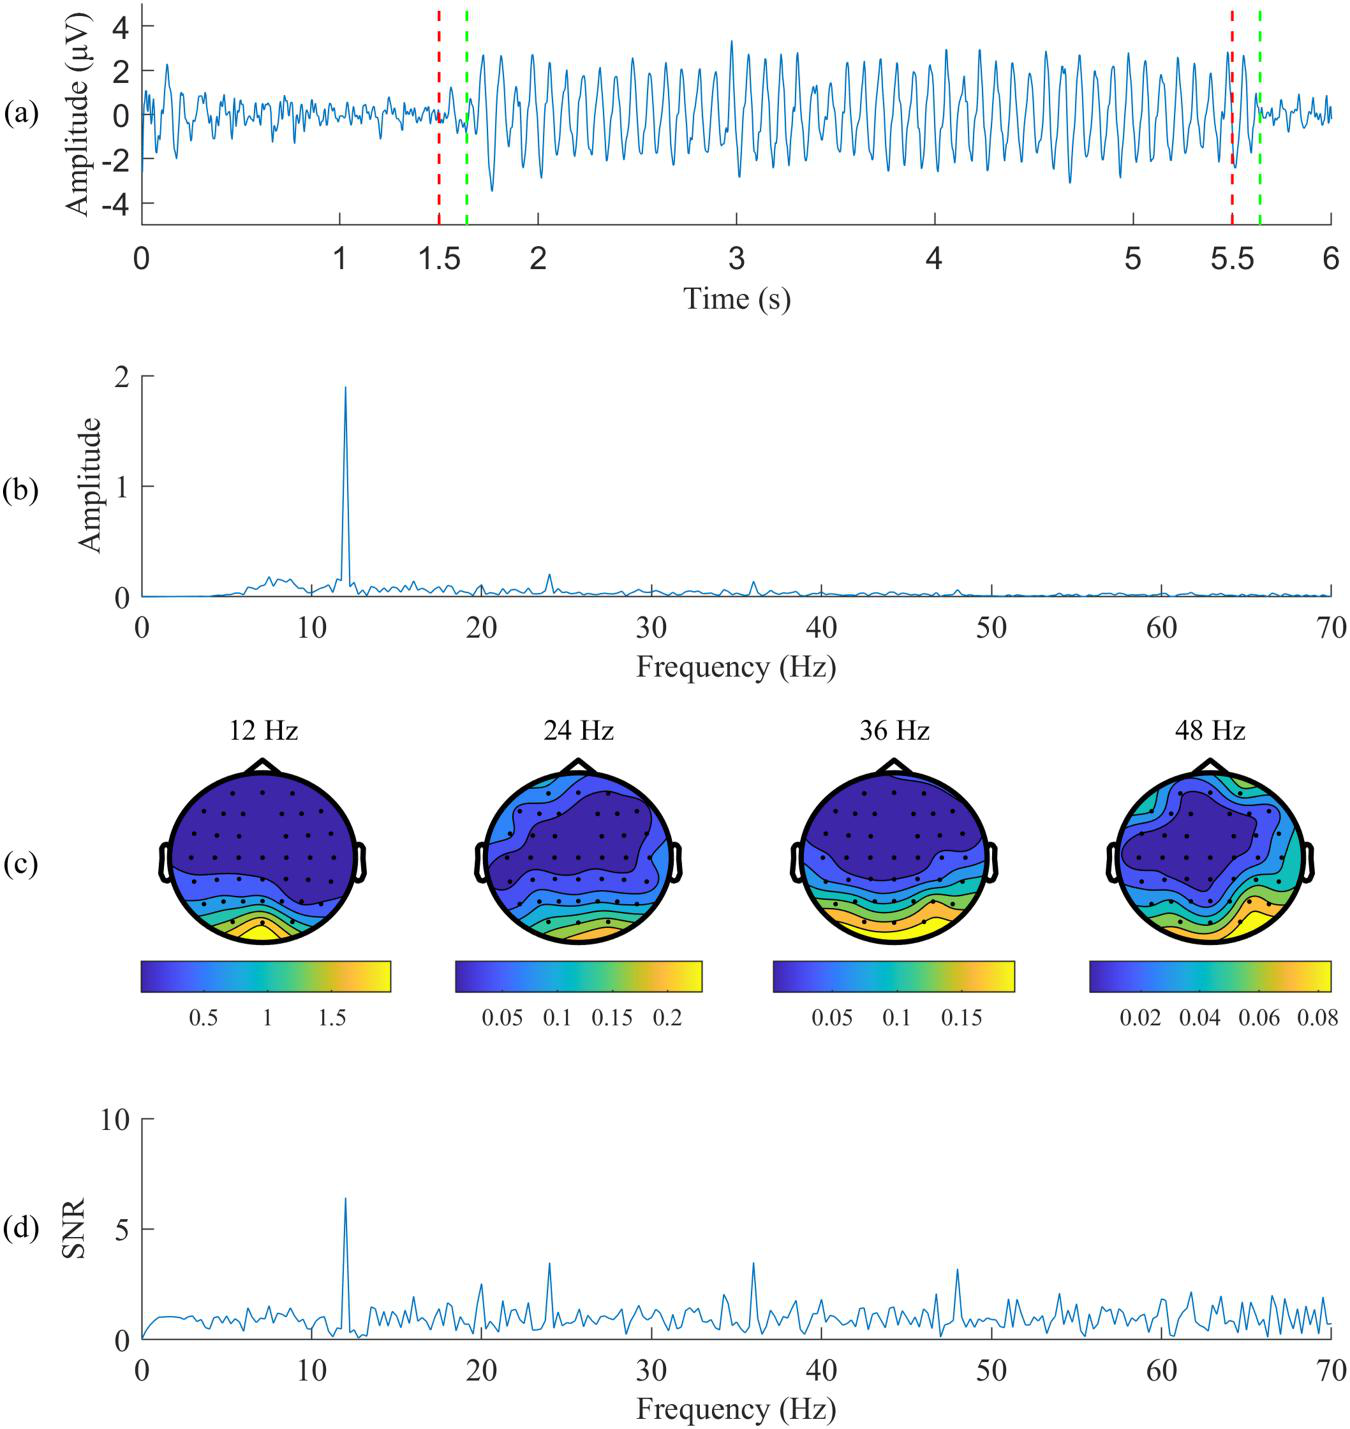
\includegraphics[width=0.72\textwidth]{figs/fig4.png}
\end{center}
\begin{en}
\textbf{Figure 4.} Signal quality analysis of the CS trials corresponding to the 12 Hz target. (a) Average temporal waveform from the Oz electrode. The red dashed lines indicate the onset and offset of the flickering. The green dashed lines indicate a visual delay of 140 ms. (b) Average amplitude spectrum. (c) Scalp maps at the fundamental, second, third, and fourth harmonic frequencies (12 Hz, 24 Hz, 36 Hz, and 48 Hz respectively). (d) Average SNR of 12 Hz SSVEP.
\end{en}
\begin{zh}
\textbf{图 4.} 12 Hz 目标对应 CS 试次的信号质量分析。(a) Oz 电极的平均时域波形，红色虚线表示闪烁的起止，绿色虚线表示 140 ms 的视觉延迟；(b) 平均幅值谱；(c) 基波、二次、三次与四次谐波频率（分别为 12 Hz、24 Hz、36 Hz 与 48 Hz）处的头皮地形图；(d) 12 Hz SSVEP 的平均 SNR。
\end{zh}

\subsection{SSVEP 频率识别（Recognition of SSVEP Frequencies）}
\begin{en}
To evaluate the recognition performance of SSVEP frequencies for the dataset, this study adopted three frequency recognition algorithms, i.e., FBCCA, TRCA and eTRCA, to classify the EEG data from the 8-class CS task for all the subjects. Nine electrodes including Pz, PO7, PO3, POz, PO4, PO8, O1, Oz and O2 were used for the following analysis. The three algorithms were evaluated using a 12-fold cross-validation, each fold consisting of 11 training trials and 1 test trial for each stimulation frequency. In this study, the number of sub-bands was set to 4, and the passbands of filter banks was set from $m\times8-2$ Hz to 80 Hz. Here, $m=1,2,3,4$ indicates the index of filter bank. These algorithms recognized the target frequency according to the weighted sum of the correlation coefficients between the sub-band components and a template data. The FBCCA algorithm constructed the template using sinusoidal and cosine reference, while the TRCA and eTRCA algorithms constructed the templates based on the training set. Other parameters for these three algorithms were the same with references [7, 8].
\end{en}
\begin{zh}
为评估数据集的 SSVEP 频率识别性能，本研究采用 FBCCA、TRCA 与 eTRCA 三种频率识别算法，对所有被试 8 分类 CS 任务的 EEG 数据进行分类。以下分析使用了 Pz、PO7、PO3、POz、PO4、PO8、O1、Oz 和 O2 共九个电极。三种算法均采用 12 折交叉验证（12-fold cross-validation）进行评估，每折中每个刺激频率包含 11 个训练试次和 1 个测试试次。本研究将子带（sub-band）数量设为 4，滤波器组的通带设为从 $m\times8-2$ Hz 至 80 Hz，其中 $m=1,2,3,4$ 表示滤波器组序号。这些算法根据子带成分与模板数据之间相关系数的加权和来识别目标频率。FBCCA 算法使用正弦与余弦参考信号构建模板，而 TRCA 与 eTRCA 算法基于训练集构建模板。三种算法的其他参数与文献 [7, 8] 相同。
\end{zh}

\begin{en}
Figure 5 shows the classification accuracies of the three algorithms with data lengths from 1 s to 4 s. The results showed that the average accuracies were improved with the increase of the data length. When the data length was set to 4 s, the FBCCA, eTRCA and TRCA algorithms obtained average accuracies of 93.49\%, 79.47\% and 73.00\%, respectively. Among the three algorithms, the FBCCA algorithm achieved the highest accuracies regardless of data length, while the TRCA and eTRCA algorithms delivered larger inter-subject variability.
\end{en}
\begin{zh}
图 5 展示了数据长度为 1 s 至 4 s 时三种算法的分类准确率。结果表明，平均准确率随数据长度的增加而提升。当数据长度为 4 s 时，FBCCA、eTRCA 与 TRCA 算法的平均准确率分别为 93.49\%、79.47\% 和 73.00\%。在三种算法中，无论数据长度如何，FBCCA 算法均取得最高准确率，而 TRCA 与 eTRCA 算法则表现出更大的被试间差异。
\end{zh}

\begin{en}
Figure 6 shows the ITRs of the three algorithms with data lengths from 1 s to 4 s. The results showed that all these algorithms obtained the highest ITRs with data length of 1 s. When the data length was set to 1 s, the FBCCA, eTRCA and TRCA algorithms obtained average ITRs of 43.8325 bits/min, 33.3243 bits/min and 29.1990 bits/min. As shown in Figure 6 (b)--(d), the eTRCA and TRCA algorithms delivered larger inter-subject variability than the FBCCA algorithm.
\end{en}
\begin{zh}
图 6 展示了数据长度为 1 s 至 4 s 时三种算法的 ITR。结果表明，所有算法在数据长度为 1 s 时取得最高 ITR。当数据长度为 1 s 时，FBCCA、eTRCA 与 TRCA 算法的平均 ITR 分别为 43.8325 bits/min、33.3243 bits/min 和 29.1990 bits/min。如图 6(b)--(d) 所示，eTRCA 与 TRCA 算法比 FBCCA 算法表现出更大的被试间差异。
\end{zh}

\begin{center}
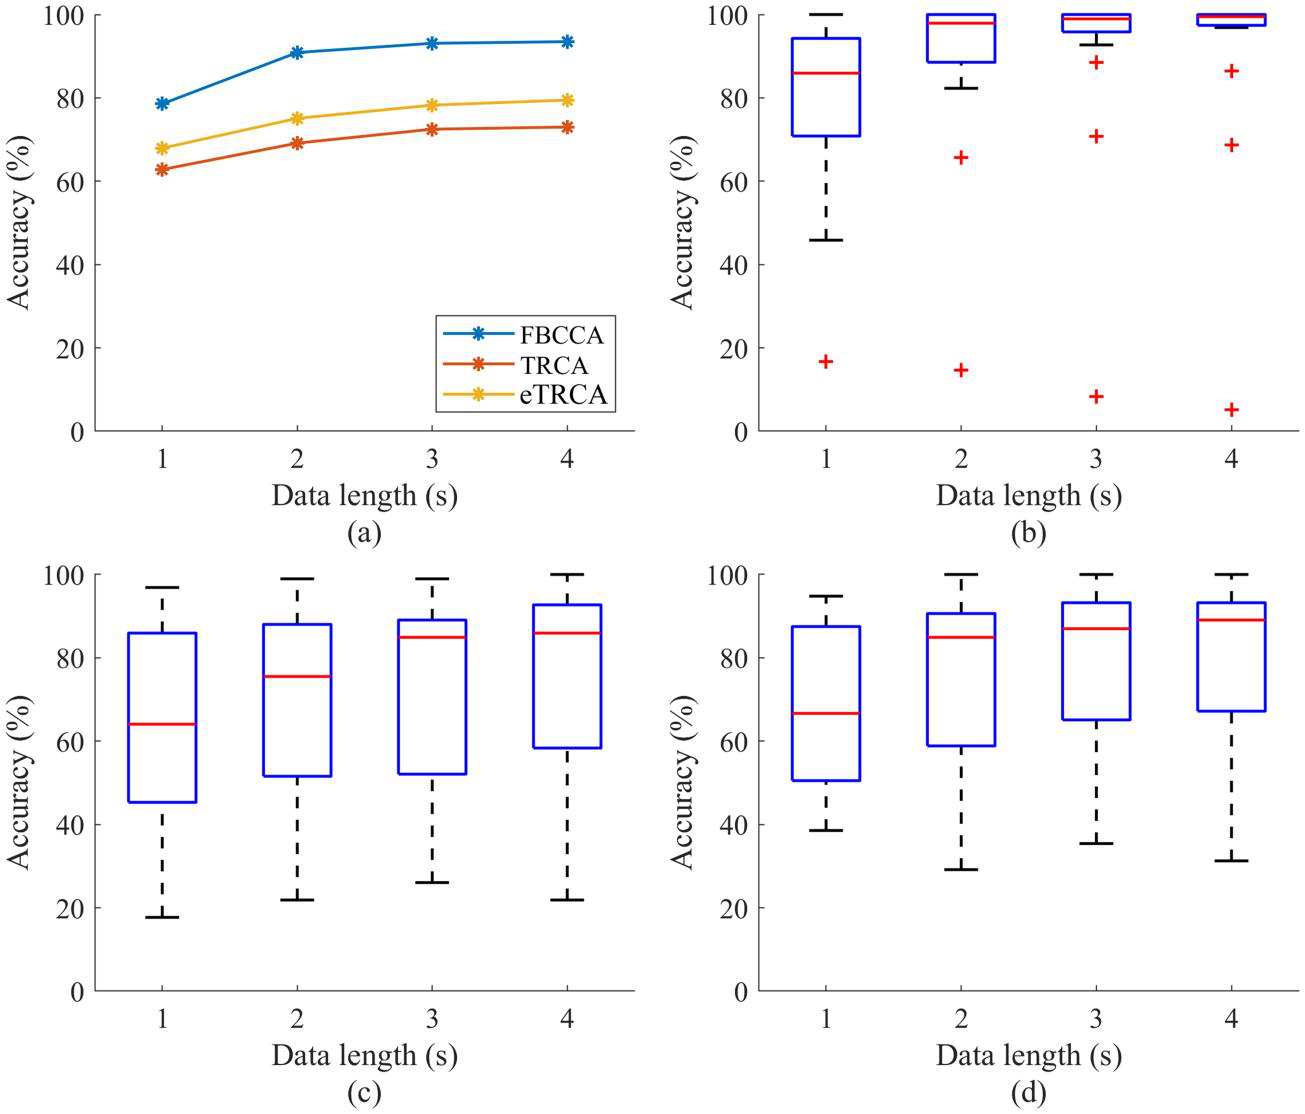
\includegraphics[width=0.9\textwidth]{figs/fig5.png}
\end{center}
\begin{en}
\textbf{Figure 5.} Classification accuracies of the FBCCA, TRCA and eTRCA algorithms with data lengths ranging from 1 s to 4 s in recognition of SSVEP frequencies. (a) Comparison of the accuracy between different algorithms. (b) Boxplot of the classification result for the FBCCA algorithm. (c) Boxplot of the classification result for the TRCA algorithm. (d) Boxplot of the classification result for the eTRCA algorithm.
\end{en}
\begin{zh}
\textbf{图 5.} 数据长度为 1--4 s 时，FBCCA、TRCA 与 eTRCA 算法在 SSVEP 频率识别中的分类准确率。(a) 不同算法准确率对比；(b) FBCCA 算法分类结果箱线图；(c) TRCA 算法分类结果箱线图；(d) eTRCA 算法分类结果箱线图。
\end{zh}

\begin{center}
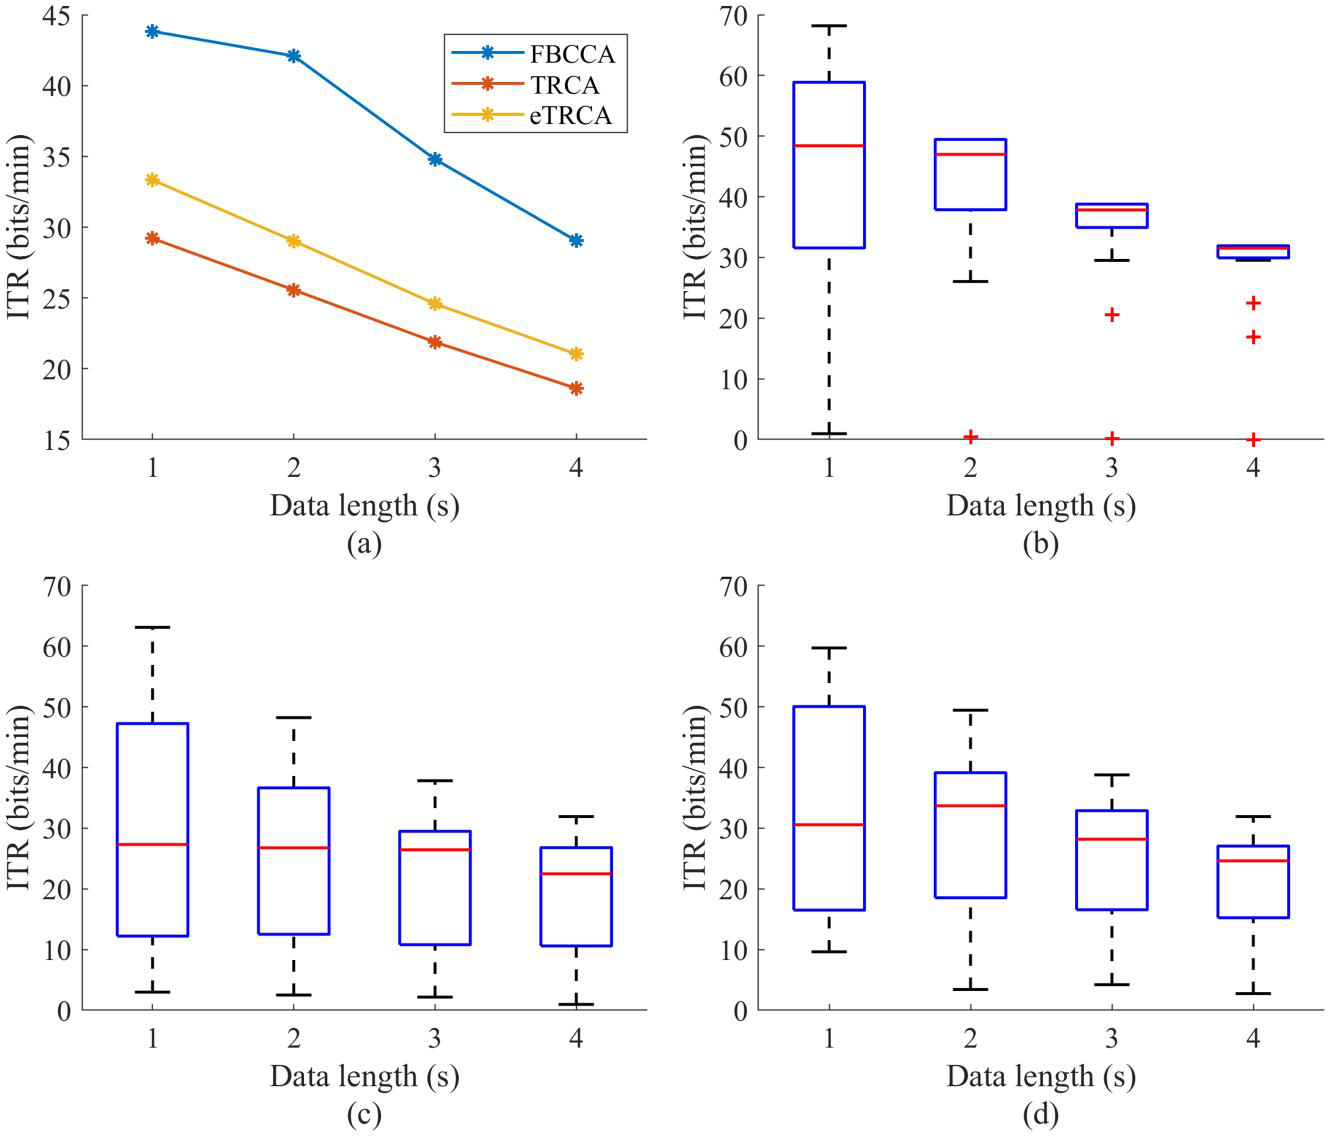
\includegraphics[width=0.9\textwidth]{figs/fig6.png}
\end{center}
\begin{en}
\textbf{Figure 6.} ITRs of the FBCCA, TRCA and eTRCA algorithms with data lengths ranging from 1 s to 4 s in recognition of SSVEP frequencies. (a) Comparison of the ITR between different algorithms. (b) Boxplot of the ITR for the FBCCA algorithm. (c) Boxplot of the ITR for the TRCA algorithm. (d) Boxplot of the ITR for the eTRCA algorithm.
\end{en}
\begin{zh}
\textbf{图 6.} 数据长度为 1--4 s 时，FBCCA、TRCA 与 eTRCA 算法在 SSVEP 频率识别中的 ITR。(a) 不同算法 ITR 对比；(b) FBCCA 算法 ITR 箱线图；(c) TRCA 算法 ITR 箱线图；(d) eTRCA 算法 ITR 箱线图。
\end{zh}

\subsection{CS 与 NS 状态的分类（Classification between CS and NS States）}
\begin{en}
In this study, we evaluated the classification performance of the dataset between the CS task and the three NS tasks. The data length was set to 1 s for the following analysis. For the CS task, 1-s data epochs were extracted from 0.14 s to 1.14 s for each trail (0 indicates the stimuli onset). For the NS tasks, the data trials were split into non-overlapping 1-s data epochs. Therefore, a total of 96 trials were acquired for each of the CS, NS1, NS2 and NS3 tasks. This study used the IFB-OCN, FS-eTRCA, and FS-eTRCA\&FBCCA algorithms to evaluate the classification performance between these tasks.
\end{en}
\begin{zh}
本研究评估了数据集在 CS 任务与三种 NS 任务之间的分类性能。以下分析中数据长度设为 1 s。对于 CS 任务，从每个试次的 0.14 s 至 1.14 s（0 表示刺激起始）提取 1 s 数据片段；对于 NS 任务，将数据试次切分为不重叠的 1 s 数据片段。因此，CS、NS1、NS2 与 NS3 每项任务各获得 96 个试次。本研究使用 IFB-OCN、FS-eTRCA 与 FS-eTRCA\&FBCCA 算法评估这些任务之间的分类性能。
\end{zh}

\begin{en}
The IFB-OCN algorithm discriminated the CS and NS using the EEG data from a single channel at frontal area [12]. It divided the pre-processed data into multiple sub-bands, and selected the first three bands with the highest accuracies for feature extraction. The OCN features were extracted for each sub-band and were integrated for the final decisions. This study selected channel Fp1 and used a linear support vector machine (SVM) classifier [24] for classification. The FS-eTRCA algorithm extracted the correlation coefficient features between EEG data and the templates for the eight stimuli using the eTRCA algorithm. It identified the stimulation frequency by selecting the maximum coefficient, and trained linear discriminant analysis (LDA) [25] classifiers to discriminate between the corresponding CS and the NS. The FS-eTRCA\&FBCCA algorithm was developed based on FS-eTRCA and adopted an additional FBCCA algorithm for feature extraction. The correlation coefficients extracted by eTRCA and FBCCA were combined as the final features for classification.
\end{en}
\begin{zh}
IFB-OCN 算法利用额区单通道的 EEG 数据区分 CS 与 NS [12]。它将预处理后的数据划分为多个子带，并选取准确率最高的前三个子带用于特征提取；对每个子带提取 OCN 特征，再将其整合用于最终决策。本研究选取 Fp1 通道，并使用线性支持向量机（support vector machine, SVM）分类器 [24] 进行分类。FS-eTRCA 算法使用 eTRCA 算法提取 EEG 数据与八个刺激模板之间的相关系数特征；通过选取最大相关系数来识别刺激频率，并训练线性判别分析（linear discriminant analysis, LDA）[25] 分类器来区分相应的 CS 与 NS。FS-eTRCA\&FBCCA 算法在 FS-eTRCA 基础上发展而来，额外采用 FBCCA 算法进行特征提取，将由 eTRCA 与 FBCCA 提取的相关系数合并作为最终分类特征。
\end{zh}

\begin{en}
The classification performance of the three algorithms were evaluated using a 12-fold cross-validation. Different from the evaluation process of recognition of SSVEP frequencies, this evaluation trained and tested the algorithms using EEG data from the CS task and each of the three NS tasks, respectively. The IFB-OCN algorithm classified two classes of the CS and NS, while the FS-eTRCA and FS-eTRCA\&FBCCA algorithms discriminated nine classes, including a NS and eight stimulation frequencies.
\end{en}
\begin{zh}
三种算法的分类性能均通过 12 折交叉验证进行评估。与 SSVEP 频率识别的评估过程不同，该评估分别使用 CS 任务与三种 NS 任务各自的数据训练和测试算法。IFB-OCN 算法进行 CS 与 NS 的二分类，而 FS-eTRCA 与 FS-eTRCA\&FBCCA 算法进行九分类，包括一个 NS 和八个刺激频率。
\end{zh}

\begin{en}
Figure 7 shows the classification accuracies of the three algorithms for discriminating between the CS and the three NSs. The results showed that the IFB-OCN algorithm achieved average accuracies of 70.51\%, 72.35\% and 69.34\% in separating the CS with NS1, NS2 and NS3, respectively. The FS-eTRCA algorithm obtained an average accuracy of 67.64\%, 66.47\% and 65.34\% in classifying nine classes including eight stimulation frequencies and a NS. The FS-eTRCA\&FBCCA algorithm outperformed the FS-eTRCA by incorporating the FBCCA features and achieved average accuracies of 76.39\%, 75.35\% and 75.02\%.
\end{en}
\begin{zh}
图 7 展示了三种算法区分 CS 与三种 NS 的分类准确率。结果表明，IFB-OCN 算法在区分 CS 与 NS1、NS2、NS3 时平均准确率分别为 70.51\%、72.35\% 和 69.34\%；FS-eTRCA 算法在包含八个刺激频率和一个 NS 的九分类中平均准确率分别为 67.64\%、66.47\% 和 65.34\%；FS-eTRCA\&FBCCA 算法通过引入 FBCCA 特征优于 FS-eTRCA，平均准确率分别达到 76.39\%、75.35\% 和 75.02\%。
\end{zh}

\begin{center}
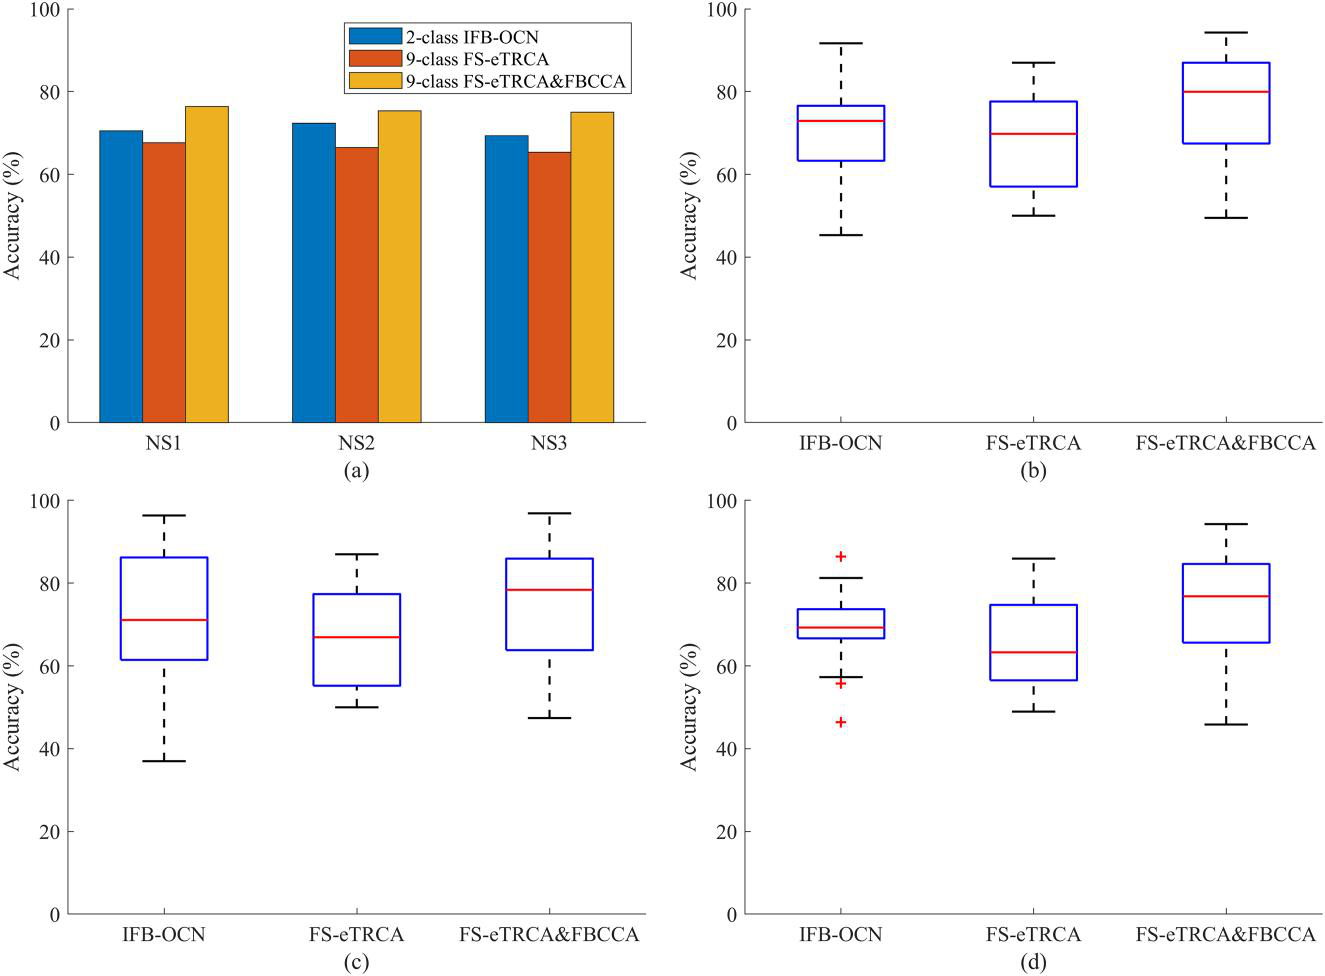
\includegraphics[width=0.9\textwidth]{figs/fig7.png}
\end{center}
\begin{en}
\textbf{Figure 7.} Classification accuracies of the IFB-OCN, FS-eTRCA and FS-eTRCA\&FBCCA algorithms with data length of 1 s in classification between CS and NS. (a) Comparison of the classification accuracy between different algorithms. (b) Boxplot of the discrimination accuracy between the CS and NS1. (c) Boxplot of the discrimination accuracy between the CS and NS2. (d) Boxplot of the discrimination accuracy between the CS and NS3.
\end{en}
\begin{zh}
\textbf{图 7.} 数据长度为 1 s 时，IFB-OCN、FS-eTRCA 与 FS-eTRCA\&FBCCA 算法在 CS 与 NS 分类中的准确率。(a) 不同算法分类准确率对比；(b) CS 与 NS1 区分准确率箱线图；(c) CS 与 NS2 区分准确率箱线图；(d) CS 与 NS3 区分准确率箱线图。
\end{zh}

% ================= 5 讨论 =================
\section{讨论（Discussions）}
\begin{en}
As the existing SSVEP-related datasets usually record a small amount of NS trials with short duration, the motivation of this article is to publish an open-source dataset with large quantity and variety of NS data to facilitate the asynchronous SSVEP research. This dataset incorporates SSVEP data and three other types of NS data, providing rich potential for further exploration. Firstly, the dataset can be used for synchronous SSVEP research. The CS data is recorded corresponding to eight stimulation frequencies, and is suitable to investigate the algorithms for feature extraction, parameter optimization and classification [26]. Secondly, the dataset can be used for discrimination studies between CS and NS. In addition, the three types of NS data benefit the robustness validation of the discrimination algorithms. Thirdly, the dataset facilitates the investigation of relationships between different CS and NS.
\end{en}
\begin{zh}
由于现有 SSVEP 相关数据集通常只记录数量少、时长短的 NS 试次，本文的动机在于发布一个包含大量且多样化 NS 数据的开源数据集，以促进异步 SSVEP 研究。该数据集包含 SSVEP 数据以及三种其他类型的 NS 数据，为进一步探索提供了丰富潜力。首先，该数据集可用于同步 SSVEP 研究：CS 数据对应八个刺激频率记录，适合用于研究特征提取、参数优化与分类算法 [26]。其次，该数据集可用于 CS 与 NS 的区分研究；此外，三种类型的 NS 数据有助于验证区分算法的鲁棒性。第三，该数据集有助于研究不同 CS 与 NS 之间的关系。
\end{zh}

\begin{en}
However, there are still two limitations to our present work. On one hand, the influence factors in subject recruitment such as age group and education background are not yet considered in this dataset. Larger sample size and diverse of subjects will be recruited in our future data collection works. On the other hand, the experimental paradigm of this dataset is designed mainly for offline asynchronous studies. In these studies, the EEG data separately acquired from the CS and NS trials can be used for investigation of features and algorithms. But for online studies requiring continuous acquisition of all the states, this dataset is currently not suitable.
\end{en}
\begin{zh}
然而，本工作仍存在两点局限。一方面，本数据集尚未考虑被试招募中的影响因素，如年龄段与教育背景；在未来的数据采集工作中，我们将招募更大样本量、更多样化的被试。另一方面，本数据集的实验范式主要面向离线异步研究而设计——此类研究中，分别从 CS 与 NS 试次采集的 EEG 数据可用于特征与算法研究；但对于需要连续采集全部状态的在线研究，本数据集目前并不适用。
\end{zh}

\begin{en}
To verify the data quality of this dataset, SSVEP recognition was conducted using three methods with a time range from 1 s to 4 s. The FBCCA algorithm outperformed the TRCA and eTRCA algorithms in terms of accuracy (Figure 6) and ITR (Figure 7). One possible reason for this is that the stimulation phases were the same for all stimuli in this dataset. As the TRCA and eTRCA algorithms utilized both frequency and phase information for SSVEP recognition, a lack of phase variance reduced their classification performance. This also holds true for the classification between CS and NS, where the FS frame based on FBCCA and eTRCA outperformed the eTRCA-based FS frame.
\end{en}
\begin{zh}
为验证本数据集的数据质量，使用三种方法在 1 s 至 4 s 的时间范围内进行了 SSVEP 识别。FBCCA 算法在准确率与 ITR 方面均优于 TRCA 与 eTRCA 算法。一个可能的原因是本数据集中所有刺激的相位相同：由于 TRCA 与 eTRCA 算法同时利用频率与相位信息进行 SSVEP 识别，缺乏相位差异降低了其分类性能。这一点同样适用于 CS 与 NS 之间的分类——基于 FBCCA 与 eTRCA 的 FS 框架优于仅基于 eTRCA 的 FS 框架。
\end{zh}
\tnote{原文写作``accuracy (Figure 6) and ITR (Figure 7)''，按上下文应分别对应图 5 与图 6，疑为原文笔误，译文已作相应调整。}

\begin{en}
In our future work, the dataset will be improved in the following aspects. Firstly, we will enlarge data recordings from a broader range of subjects to create a more generalized dataset. Additional factors will be considered during subject recruitment, such as age, education background and gender. Secondly, we will incorporate data recordings from different days of the same subject to facilitate investigation of the intra-individual variability. Thirdly, our future work will design experimental protocols for continuous acquisition of all CS and NSs, and publish dataset for evaluation of algorithms' online performance.
\end{en}
\begin{zh}
在未来的工作中，我们将从以下方面改进该数据集。首先，我们将扩大数据采集的被试范围，构建更具泛化性的数据集，并在被试招募时考虑年龄、教育背景与性别等更多因素。其次，我们将纳入同一被试不同日期的数据记录，以便研究个体内变异性。第三，我们未来的工作将设计可连续采集全部 CS 与 NS 的实验方案，并发布数据集以评估算法的在线性能。
\end{zh}

% ================= 6 结论 =================
\section{结论（Conclusion）}
\begin{en}
The presented study introduces a dataset for studying asynchronous SSVEP-based BCI. This dataset includes four distinct data types: CS data based on SSVEP at frequencies of 8, 9, 10.5, 11, 12, 13, 14 and 15 Hz, as well as three types of NS data. Through analysis of temporal waveforms, amplitude waveforms, SNR in the frequency domain, and spectral amplitude distribution in the spatial domain, we validated the SSVEP signal quality of our dataset. Moreover, the results of frequency recognition using FBCCA, TRCA, and eTRCA methods demonstrated the effectiveness of this dataset in SSVEP classification, and the results of state classification using IFB-OCN, FS-eTRCA and FS-eTRCA\&FBCCA methods demonstrated effectiveness of this dataset in discrimination between CS and NS.
\end{en}
\begin{zh}
本研究介绍了一个用于研究基于异步 SSVEP 的 BCI 的数据集。该数据集包含四种不同的数据类型：基于 8、9、10.5、11、12、13、14 与 15 Hz SSVEP 的 CS 数据，以及三种类型的 NS 数据。通过分析时域波形、幅值波形、频域 SNR 以及空间域的频谱幅值分布，我们验证了数据集的 SSVEP 信号质量。此外，使用 FBCCA、TRCA 与 eTRCA 方法进行频率识别的结果证明了该数据集在 SSVEP 分类中的有效性；使用 IFB-OCN、FS-eTRCA 与 FS-eTRCA\&FBCCA 方法进行状态分类的结果证明了该数据集在 CS 与 NS 区分中的有效性。
\end{zh}

% ================= 声明 =================
\section*{利益冲突声明（Disclosure Statement）}
\begin{en}
The authors report there are no competing interests to declare.
\end{en}
\begin{zh}
作者声明不存在需要披露的利益冲突。
\end{zh}

\section*{基金资助（Funding）}
\begin{en}
This research was supported by the National Key R\&D Program of China (2022YFE0140400), National Natural Science Foundation of China (62376241), and S\&T Program of Hebei (236Z2001G).
\end{en}
\begin{zh}
本研究受国家重点研发计划（2022YFE0140400）、国家自然科学基金（62376241）与河北省科技计划（236Z2001G）资助。
\end{zh}

\section*{数据可用性声明（Data Availability Statement）}
\begin{en}
The data that support the findings of this study are openly available in figshare at \url{https://doi.org/10.6084/m9.figshare.24906300.v3}, reference number [21].
\end{en}
\begin{zh}
支持本研究结论的数据已在 figshare 平台开放获取：\url{https://doi.org/10.6084/m9.figshare.24906300.v3}（参考文献 [21]）。
\end{zh}

% ================= 参考文献 =================
\section*{参考文献（References）}
\noindent\textcolor{gray}{\small 参考文献保留英文原文，便于检索核对。}
\emergencystretch=3em
\sloppy

\begin{enumerate}[label={[\arabic{enumi}]}, leftmargin=3.2em, itemsep=2pt]
\item Wang Y, Gao X, Hong B, et al. Brain-computer interfaces based on visual evoked potentials. IEEE Eng Med Biol Mag. 2008;27(5):64--71. doi: 10.1109/MEMB.2008.923958.
\item Zhao J, Li W, Li M. Comparative study of SSVEP- and P300-based models for the telepresence control of humanoid robots. PLoS One. 2015;10(11):e0142168. doi: 10.1371/journal.pone.0142168.
\item Chen X, Chen Z, Gao S, et al. Brain--computer interface based on intermodulation frequency. J Neural Eng. 2013;10(6):066009. doi: 10.1088/1741-2560/10/6/066009.
\item Ortner R, Guger C, Prueckl R, et al. SSVEP based brain-computer interface for robot control. In: Miesenberger K, Klaus J, Zagler W, Karshmer A, editors. Computers helping people with special needs. Berlin (Heidelberg): Springer; 2010. p. 85--90.
\item G\"uneysu A, Akin HL. An SSVEP based BCI to control a humanoid robot by using portable EEG device. Annu Int Conf IEEE Eng Med Biol Soc. 2013;2013:6905--6908. doi: 10.1109/EMBC.2013.6611145.
\item Yao H, Liu K, Deng X, et al. FB-EEGNet: a fusion neural network across multi-stimulus for SSVEP target detection. J Neurosci Method. 2022;379:109674. doi: 10.1016/j.jneumeth.2022.109674.
\item Nakanishi M, Wang Y, Chen X, et al. Enhancing detection of SSVEPs for a high-speed brain speller using task-related component analysis. IEEE Trans Biomed Eng. 2018;65(1):104--112. doi: 10.1109/TBME.2017.2694818.
\item Chen X, Wang Y, Gao S, et al. Filter bank canonical correlation analysis for implementing a high-speed SSVEP-based brain-computer interface. J Neural Eng. 2015;12(4):046008. doi: 10.1088/1741-2560/12/4/046008.
\item Wong CM, Wan F, Wang B, et al. Learning across multi-stimulus enhances target recognition methods in SSVEP-based BCIs. J Neural Eng. 2020;17(1):016026. doi: 10.1088/1741-2552/ab2373.
\item Pan Y, Chen J, Zhang Y, et al. An efficient CNN-LSTM network with spectral normalization and label smoothing technologies for SSVEP frequency recognition. J Neural Eng. 2022;19(5):056014. doi: 10.1088/1741-2552/ac8dc5.
\item Pan J, Li Y, Zhang R, et al. Discrimination between control and idle states in asynchronous SSVEP-based brain switches: a pseudo-key-based approach. IEEE Trans Neural Syst Rehabil Eng. 2013;21(3):435--443. doi: 10.1109/TNSRE.2013.2253801.
\item Zhang W, Zhou T, Zhao J, et al. Recognition of the idle state based on a novel IFB-OCN method for an asynchronous brain-computer interface. J Neurosci Methods. 2020;341:108776. doi: 10.1016/j.jneumeth.2020.108776.
\item Ke Y, Du J, Liu S, et al. Enhancing detection of control state for high-speed asynchronous SSVEP-BCIs using frequency-specific framework. IEEE Trans Neural Syst Rehabil Eng. 2023;PP:1405--1417. doi: 10.1109/TNSRE.2023.3246359.
\item Wang R, Zhou T, Li Z, et al. Using oscillatory and aperiodic neural activity features for identifying idle state in SSVEP-based BCIs reduces false triggers. J Neural Eng. 2023;20(6):066032. doi: 10.1088/1741-2552/ad1054.
\item Zhang D, Huang B, Wu W, et al. An idle-state detection algorithm for SSVEP-based brain-computer interfaces using a maximum evoked response spatial filter. Int J Neural Syst. 2015;25(7):1550030. doi: 10.1142/S0129065715500306.
\item Nagel S, Sp\"uler M. Asynchronous non-invasive high-speed BCI speller with robust non-control state detection. Sci Rep. 2019;9(1):8269. doi: 10.1038/s41598-019-44645-x.
\item Wang Y, Chen X, Gao X, et al. A benchmark dataset for SSVEP-based brain--computer interfaces. IEEE Trans Neural Syst Rehabil Eng. 2017;25(10):1746--1752. doi: 10.1109/TNSRE.2016.2627556.
\item Liu B, Huang X, Wang Y, et al. BETA: a large benchmark database toward SSVEP-BCI application. Front Neurosci. 2020;14:627. doi: 10.3389/fnins.2020.00627.
\item Chevallier S. 2023. sylvchev/dataset-ssvep-exoskeleton [Internet]. [cited 2023 Dec 26]. Available from: \url{https://github.com/sylvchev/dataset-ssvep-exoskeleton}.
\item Vilic. Avi A, Dataset S. 2013. [dataset]. In: setzner [Internet]. [cited 2023 Dec 26]. Available from: \url{https://www.setzner.com/avi-ssvep-dataset/}.
\item Zhao J, Zhang Q, Wang X-R. YSU-an EEG dataset for studying asynchronous SSVEP-BCI [Internet]. figshare; 2023 [cited 2024 Oct 8]. Available from: \url{https://figshare.com/articles/dataset/YSU-an_EEG_dataset_for_studying_asynchronous_SSVEP-BCI/24906300/3}.
\item Brainard DH, Vision S. The psychophysics toolbox. Spat Vis. 1997;10(4):433--436. doi: 10.1163/156856897X00357.
\item Chen X, Chen Z, Gao S, et al. A high-ITR SSVEP-based BCI speller. Brain-Computer Interfaces. 2014;1(3-4):181--191. doi: 10.1080/2326263X.2014.944469.
\item Chang C-C, Lin C-J. LIBSVM: a library for support vector machines. ACM Trans. Intell. Syst. Technol. 2011;2(3):1--27:27. doi: 10.1145/1961189.1961199.
\item Tharwat A, Gaber T, Ibrahim A, et al. Linear discriminant analysis: A detailed tutorial. AIC. 2017;30(2):169--190. doi: 10.3233/AIC-170729.
\item Zhang H, Zhou Q-Q, Chen H, et al. The applied principles of EEG analysis methods in neuroscience and clinical neurology. Mil Med Res. 2023;10(1):67. doi: 10.1186/s40779-023-00502-7.
\end{enumerate}

\end{document}
